\documentclass{article}
\usepackage[utf8]{inputenc}
\usepackage{subcaption}
\usepackage{amsmath}
\usepackage{amssymb}
\usepackage{hyperref}
\usepackage{titlesec}
\usepackage{xcolor}
\usepackage{fancyhdr}
\usepackage{float}
\usepackage{graphicx}
\usepackage{multirow}
\usepackage[rightcaption]{sidecap}
\usepackage{verbatim}
\usepackage{listings}
\usepackage{dirtree}
\usepackage[backend=bibtex]{biblatex}
\addbibresource{references.bib}
\usepackage [ a4paper , hmargin =1.2 in , bottom =1.5 in ] { geometry }
\hypersetup{
    colorlinks=true,
    linkcolor=blue,
    filecolor=magenta,      
    urlcolor=cyan,
}

% Add header and footer code here
\pagestyle{fancy}
\lhead{Mini Game Hub}
\title{Mini Game Hub}
\author{Bipul Kumar and S.V.S. Chakri}
\date{}
% You may also add path to the images optionally
\graphicspath{{report_images/}}

\begin{document}
\maketitle
% preamble
% below line auto generates the table of contents
% thank me for your free 1 mark
\tableofcontents
\clearpage

\section{Introduction}
This is a project made by us as part of the CS108 course (Spring 2026) which includes a mini game hub consisting of three two-player board games.
\\
This game hub includes the following features:
\begin{itemize}
    \item \textbf{Authentication:} The code for this is covered in \texttt{main.sh}. \\ For starting the game, the players enter their username and password and login (If username doesn't exist they register). \\ After logging in, the game interface shows up for the games to start between the players.
    \item \textbf{Game Engine: } The code for this is covered in \texttt{game.py}. \\ This includes the main game interface as well as other menus like game over options.
    \item \textbf{Games:} Included games are modified versions of Tic-Tac-Toe, Othello and Connect Four.
\end{itemize}
\subsection{Description of Games:}
\begin{itemize}
    \item \textbf{Tic-Tac-Toe (Expanded):} This is a modified version of tic-tac-toe which has a 10 x 10 board with two players playing X or O on the board.
    \\ It requires the player to have 5 pieces in a horizontal, vertical or diagonal (consecutive) alignment to win.
    \\ The game ends in a draw if the board gets filled and no player has 5 of their pieces aligned.
    \item \textbf{Othello (Reversi):} This is the original Othello game, played on an 8 x 8 board with two black discs and two white discs in the center.
    \\ A move is valid only if it traps one or more opponent discs in a straight line between the newly placed disc and an existing own disc. If a player has no valid move then their turn is skipped.
    \\ The player with more discs of their colour when no valid moves remain wins.
    \item \textbf{Connect Four: } This game is played on a 7 x 7 board. Each player has his own designated coin and coins fall into the lowest row of each column. 
    \\ A player wins by getting 4 of their coins aligned diagonally, horizontally or vertically consecutively. The game ends in a draw if the board fills with no winner.
\end{itemize}

This Project emphasizes of design of these games as well as addition of some extra features.
\section{Running instructions}
\begin{itemize}
    \item The game requires python version 3.11 or above along with pip.
    \item Clone the project repository on your local device and move to the root directory in the terminal.
    \item \textbf{Optional:} Setup a virtual environment for installing dependencies.
    \item Install dependencies from requirements.txt
    \begin{verbatim}
        pip install -r requirements.txt
    \end{verbatim}
    \item Start the game hub by running the following command on the terminal 
    \begin{verbatim}
        bash main.sh 
    \end{verbatim}
    \item  Follow the instructions on the screen from now on.
    \item To compile the report run:
    \begin{verbatim}
        make
    \end{verbatim}
    \item To clean auxiliary files:
    \begin{verbatim}
        make clean
    \end{verbatim}
\end{itemize}

\section{Game Layout}
\subsection{Authenticator}
The Game starts with an authenticator which stores the usernames and passwords of the players of the game in \texttt{users.tsv}. The start menu is as follows:
\begin{figure}[h]
    \centering
    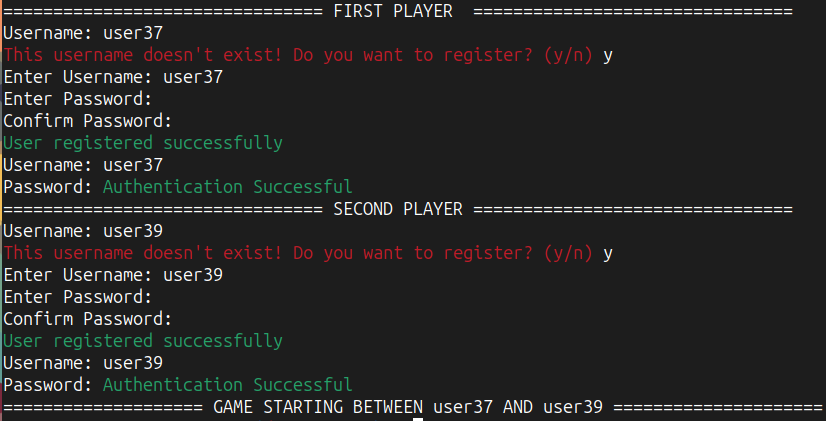
\includegraphics[width=0.7\textwidth, trim = 2 0 40 0, clip]{authenticator}
    \caption{Authenticator window in terminal}
    \label{fig:authenticator}
\end{figure}
\\
The passwords are stored in \texttt{users.tsv} using \textbf{SHA-256 hashing}\cite{sha256sum} by using \texttt{sha256sum} command in \texttt{bash}. \\
After authentication of two players is complete game between them is started by the command:
\begin{verbatim}
    python3 game.py ${USER[1]} ${USER[2]}
\end{verbatim}
\subsection{Game Engine}
The code for the game engine is included in game.py. This includes the start menu, as well as code for game over menu and the leaderboard screen. \textbf{AI generated images} have been used for the theme of \textbf{Hollow Knight} game \cite{hollowKnight}.

The start menu on start of a game between Bipul and Chakri will look as follows:
\begin{figure}[H]
    \centering
    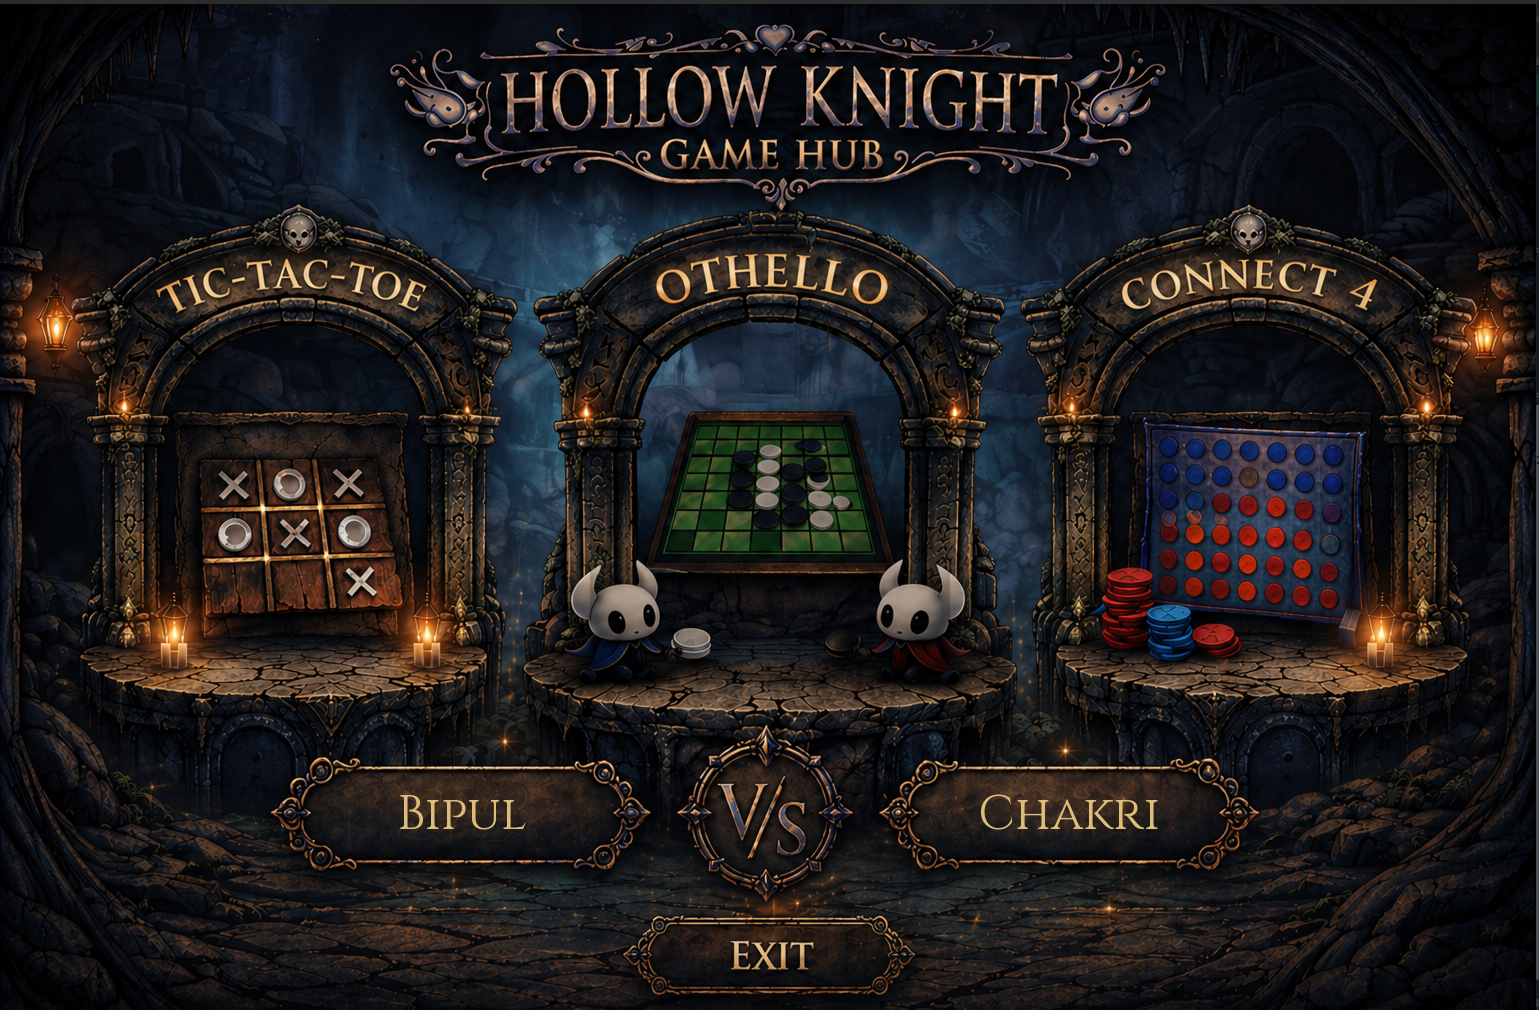
\includegraphics[width=0.7\textwidth]{start_menu}
    \caption{Authenticator window in terminal}
    \label{fig:start_menu}
\end{figure}
The users can then go on to click on the icons of the games to enter the game interface.

\subsection{Games}
In all of the following games, AI generated images have been used to make the design aesthetic and in accordance with the chosen theme of \textbf{Hollow Knight}.
\subsubsection{Tic-Tac-Toe}
This game is a modified version of usual tic-tac-toe \cite{tictactoeRules} with a 10 x 10 board. A player wins if they have 5 of their pieces (X or O) in a row (horizontally, vertically or diagonally)

The following image shows the condition of winning in this game:
\begin{figure}[H]
    \centering
    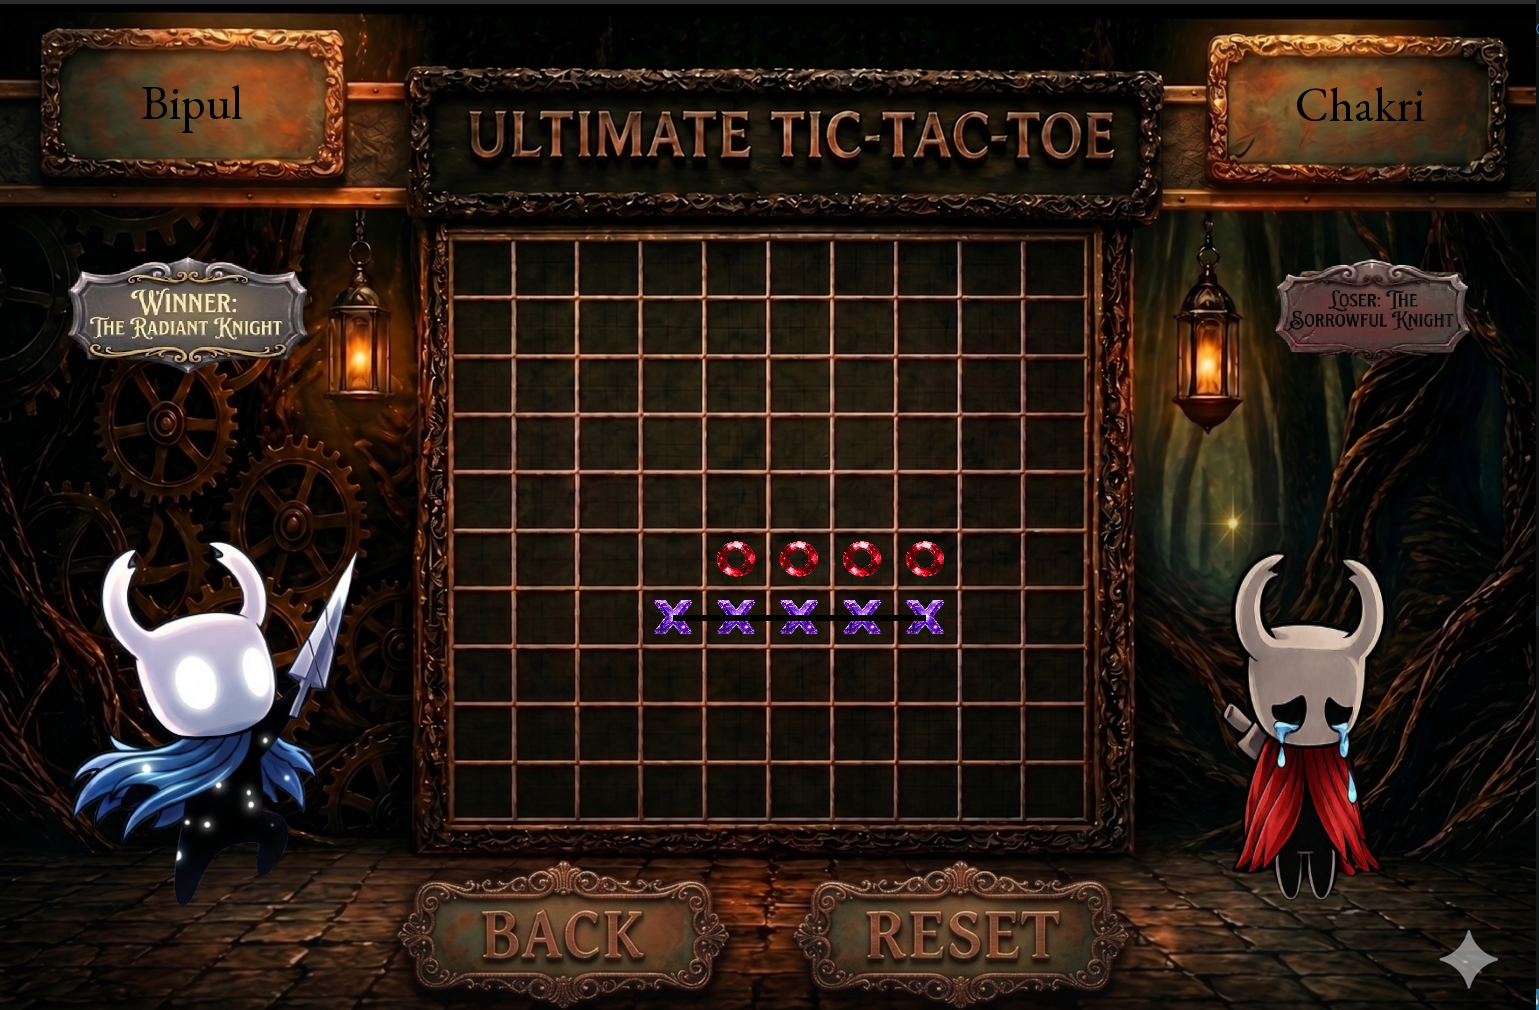
\includegraphics[width=0.7\textwidth]{tictactoe}
    \caption{Ultimate Tic-Tac-Toe}
    \label{fig:tictactoe_menu}
\end{figure}

\subsubsection{Othello (Reversi)}
This game is the usual Othello \cite{othelloReversiRules} game played using white and black pieces. 

The following image is a still in othello game:
\begin{figure}[H]
    \centering
    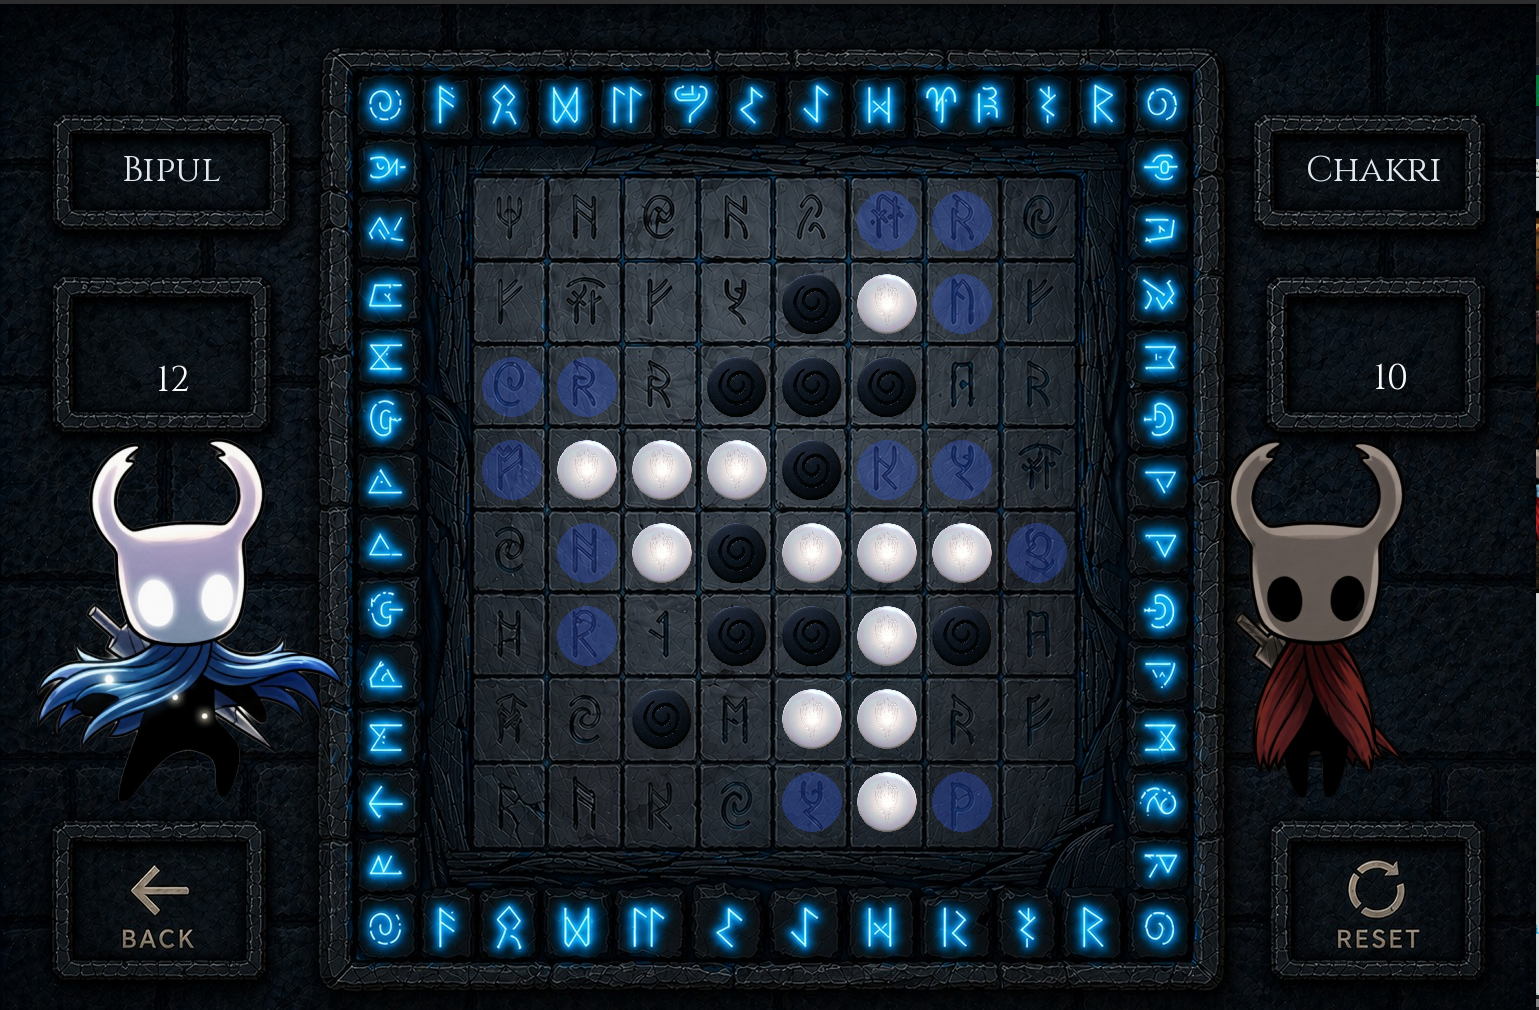
\includegraphics[width=0.7\textwidth]{othello}
    \caption{Othello game}
    \label{fig:othello}
\end{figure}
\subsubsection{Connect Four}
This game is the usual connect four \cite{connect4Rules} game played with coins falling down on a board. The theme chosen is the ancient four.
\begin{figure}[H]
    \centering
    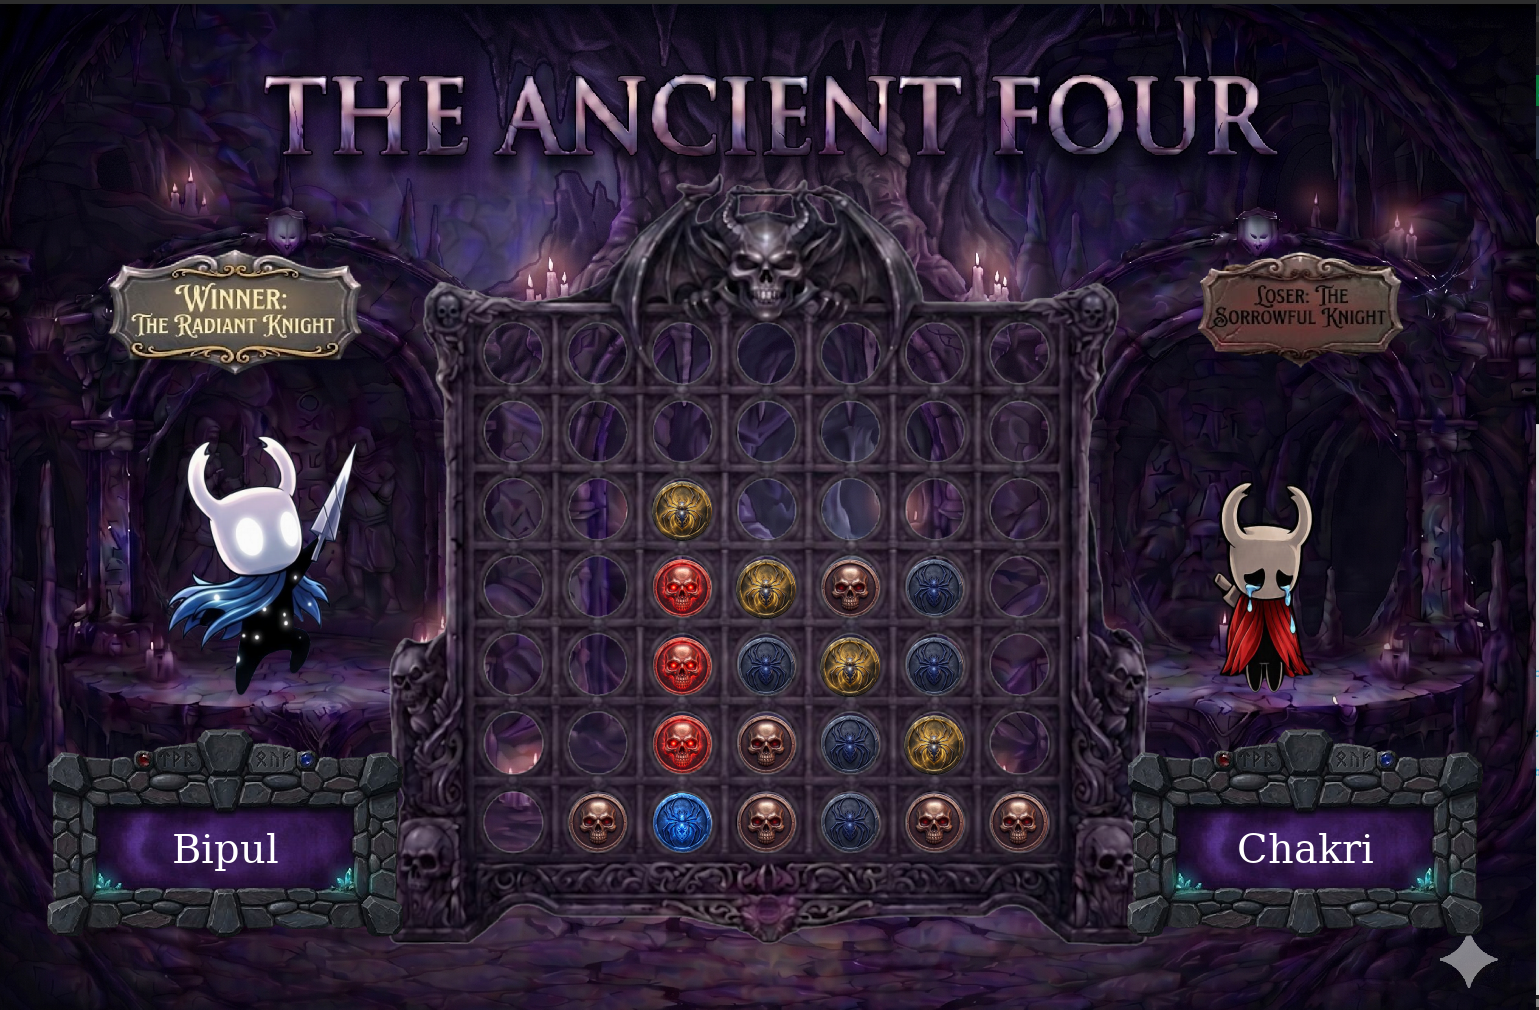
\includegraphics[width=0.7\textwidth]{connect4}
    \caption{Connect four after win}
    \label{fig:connect4}
\end{figure}
\subsection{Leaderboard and Analytics}
This is done from \texttt{leaderboard.sh} using awk\cite{awkDocs}.
\begin{figure}[H]
    \centering
    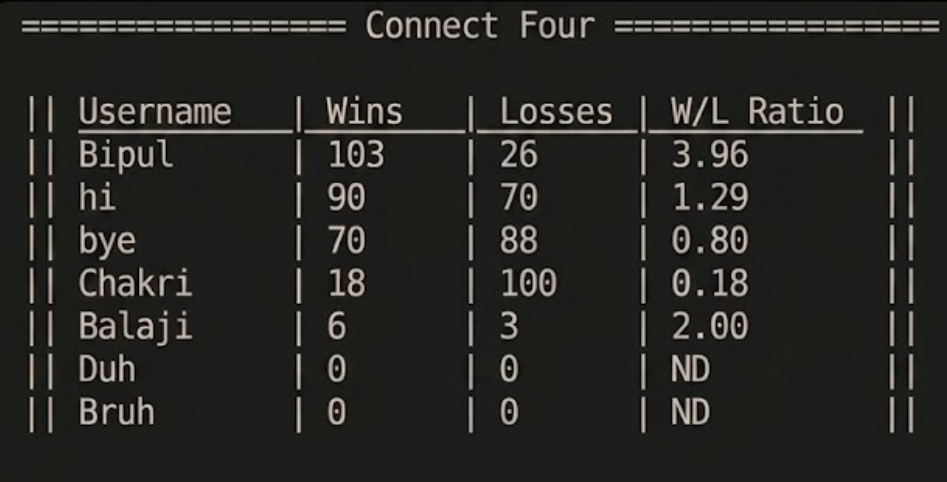
\includegraphics[width=0.7\textwidth]{leaderboard}
    \caption{Leaderbaord}
    \label{fig:leaderboard}
\end{figure}
\begin{figure}[H]
    \centering
    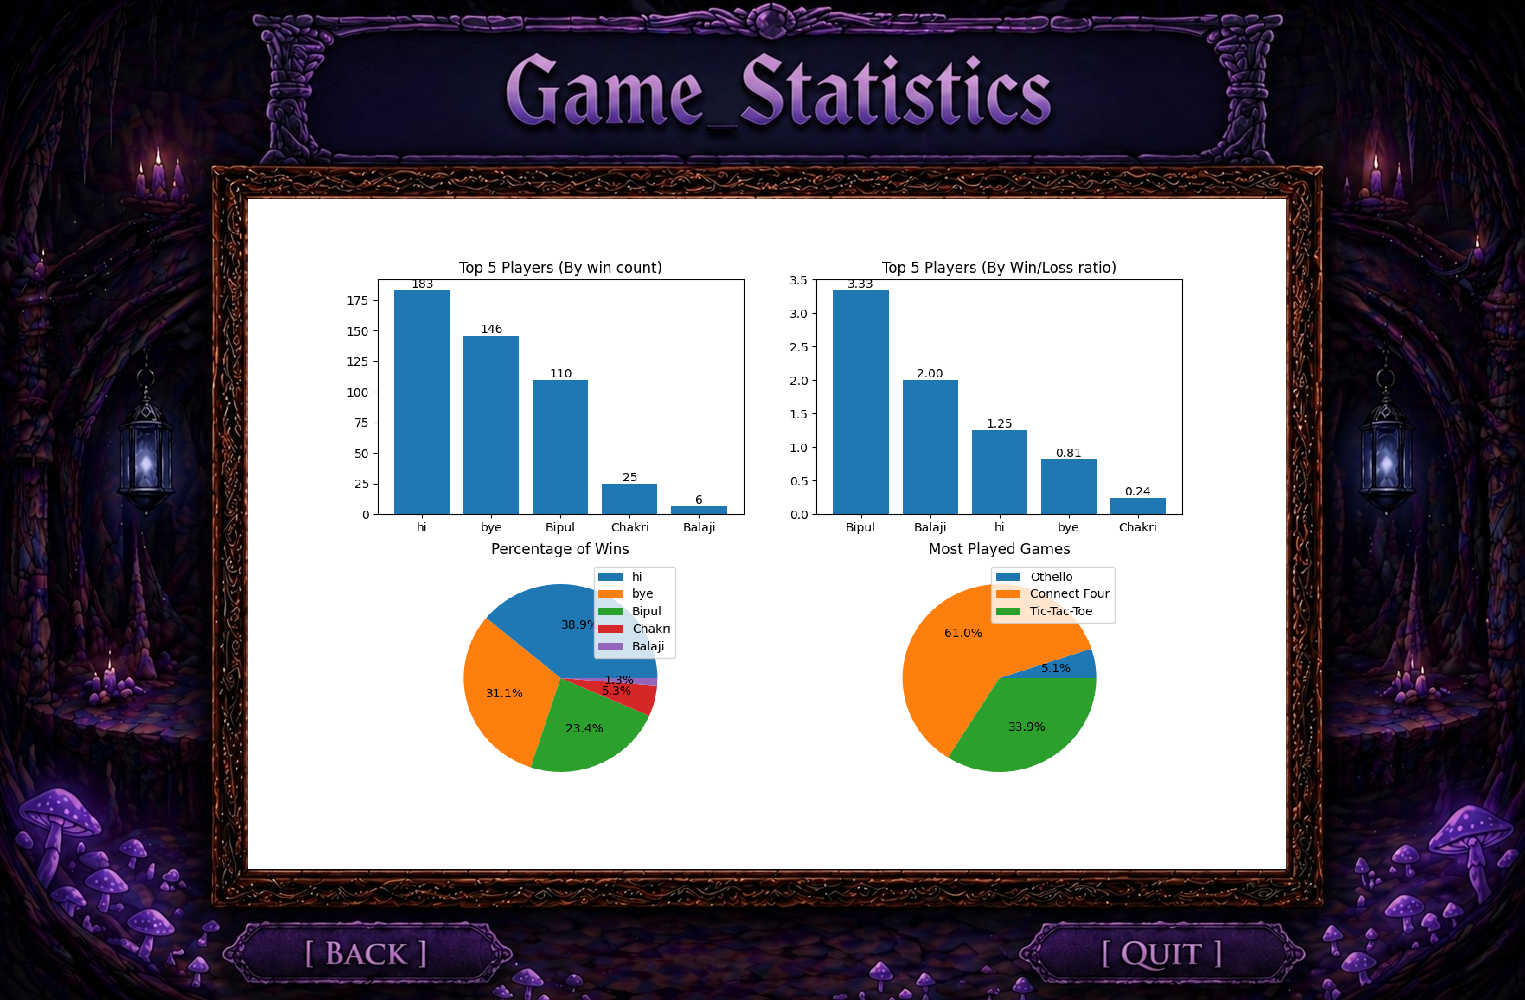
\includegraphics[width=0.7\textwidth]{charts}
    \caption{Matplotlib charts}
    \label{fig:charts}
\end{figure}
\subsection{Directory Structure}
The following directory structure has been used:
\dirtree{%
.1 PROJECT\_FOR\_CS108/.
.2 \_\_pycache\_\_/.
.2 .git/.
.2 fonts/.
.2 games/.
.2 images/.
.2 report\_images/.
.2 venv/.
.2 .gitignore.
.2 game.py.
.2 games.csv.
.2 history.csv.
.2 leaderboard.sh.
.2 main.sh.
.2 makefile.
.2 plot.png.
.2 README.md.
.2 references.bib.
.2 report.pdf.
.2 report.tex.
.2 users.tsv.
}
\section{Features and Additional Improvements}
\begin{itemize}
    \item Added back and reset features in all games
\end{itemize}
\section{Project Journey}
Could have done more things if I had 10 hours more, like adding flipping animation in othello and could have added more games
\printbibliography
\end{document}